% Very simple template for lab reports. Most common packages are already included.
\documentclass[a4paper, 11pt]{article}
\usepackage[utf8]{inputenc} % Change according your file encoding
\usepackage{graphicx}
\usepackage{url}
\usepackage{listings}
\usepackage[listings]{tcolorbox}
\usepackage{xcolor}
\usepackage{float}
\usepackage{placeins}

% Define a custom boxed listing environment
\newtcblisting{mylisting}{
  colback=gray!5!white, colframe=black!75!white,
  listing only,
  left=2mm, right=2mm, top=1mm, bottom=1mm,
  boxrule=0.5pt, arc=2mm
}

%opening
\title{Report 4 - Groupy: Group Membership Service}
\author{Lorenzo Deflorian}
\date{\today{}}

\begin{document}

\maketitle

\section{Introduction}
The main goal of the assignment was to implement a group membership service providing atomic multicasting in view synchrony while tolerating crash failures.

\section{Main problems and solutions}
\subsection{Peer pressure}
Group communication in our implementation relies on a leader-based protocol. The leader maintains a consistent view of the group membership and multicasts messages to all members. When a peer wants to join, it sends a request to the leader, who updates the group view and shares it with everyone. The view consists of two parts: the list of all \textbf{process identifiers in the group} and the list of \textbf{process identifiers at the application layer}.

Peers that are not the leader act as slaves. They forward join requests and multicast instructions to the leader and relay messages from the leader to the application layer. This setup ensures that all group members have the same view and that messages are delivered reliably, even if some processes crash.

Using our first implementation, gms1, we observe that group communication works as expected and all peers change colors in sync. However, if the leader crashes the whole system stops working.

\subsection{You have a peer in me}
To address leader crashes we use monitors to detect failures. Each peer monitors the leader and, if it detects a crash, initiates a leader election to select a new leader from the remaining members. The new leader then takes over the responsibilities of maintaining the group view and multicasting messages.

With this mechanism in place, if the leader crashes one of the slaves takes over and the system continues to function without interruption. The group members continue to change colors in sync, demonstrating that group communication is resilient to leader failures.

The implementation gms2 demonstrates these improvements and can handle leader crashes effectively.

\subsection{One two three crash}

While our gms2 implementation handles leader crashes effectively, it fails to guarantee view synchrony when failures occur during message broadcasting. To demonstrate this limitation we introduced random crashes in the broadcast function (gms2p5), where the leader might crash after sending a message to only some slaves.

This creates a critical problem: when the leader crashes mid-broadcast, some group members receive the message while others do not, leading to inconsistent states. Even after a new leader is elected, the group may remain out of sync because there is no mechanism to detect or recover from partial message delivery. This violates the reliability property of view synchrony, which requires that if any correct node delivers a message, all correct nodes must deliver it.

\begin{figure}[H]
  \centering
  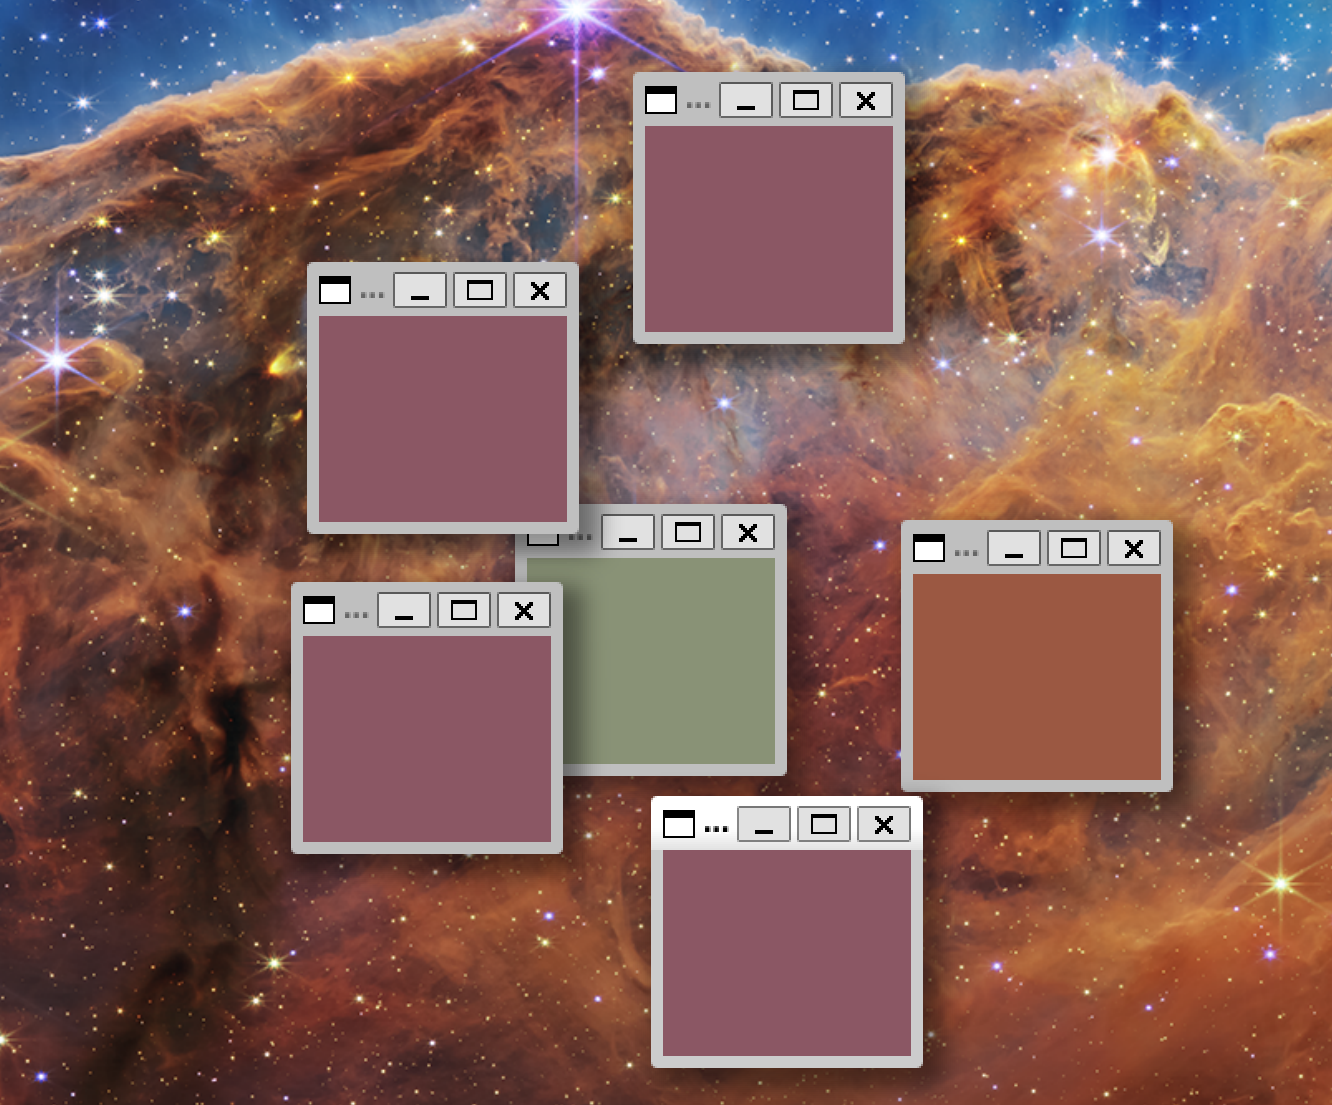
\includegraphics[width=0.7\textwidth]{imgs/out_of_sync.png}
  \caption{Peers out of sync after crash mid-broadcast.}
  \label{fig:out_of_sync}
\end{figure}

\subsection{Being a reliable peer}
From a few reasonable assumptions we can implement a more robust multicasting protocol to address the issue of leader crashes during message broadcasting.

Assuming messages are reliably delivered, if the leader sends a message to S1 and then to S2 and S2 receives it, then S1 must have received it as well. Thus, if one peer has received the message, earlier peers in the sending order should also have received it.

If the leader crashes during the multicast, some slaves might not have received the message. By keeping track of the last received message, the newly elected leader can resend the last message to all slaves, synchronizing those that missed it the first time.

To avoid applying the same message twice and advancing the application state incorrectly, we introduce sequence numbers in our messages. If a peer receives a message with a sequence number less than or equal to the last one it processed, it ignores the message.

The implementation gms3 demonstrates these improvements: it handles leader crashes while preserving view synchrony.

\subsection{Party is over}
Our implementation so far assumes that messages are reliably delivered. In a real-world scenario this might not be the case. To demonstrate the effect of message loss, I added a random drop chance in the broadcast function (gms3p5). When the leader broadcasts a message, some slaves might not receive it. A slave that misses a message will then expect an earlier sequence number and ignore subsequent messages, causing it to freeze in its state.

\subsection{Speaking up for yourself}
To address this issue we implemented the following:

The leader keeps a history buffer of the last 100 messages sent. When a slave receives a message, it checks the sequence number. If the sequence number is higher than expected, some messages were lost. The slave then sends a NACK to the leader, specifying the sequence number of the last message it received correctly. The leader resends all messages from the history buffer starting from that sequence number.

The implementation gmsX shows that sometimes messages are lost and the sync is briefly interrupted, but slaves request the missing messages and quickly catch up.

\section{Conclusions}

In this assignment we implemented a group membership service that provides atomic multicasting in view synchrony while tolerating crash failures. We started with a basic leader-based protocol and progressively enhanced it to handle leader crashes, ensure view synchrony, and deal with message loss. The final implementation demonstrates the ability to maintain a consistent group state even in the presence of failures, showcasing the robustness of our group communication system.

The NACK mechanism has low overhead and is quite efficient since it generates extra traffic only when the network is lossy.

Another approach to handle message loss is to use positive acknowledgments, where each slave acknowledges the receipt of each message. However, this would generate much more traffic and would not scale well with a large number of slaves.

\subsection{Leader crash and lost history}
Both approaches assume the leader's history is intact when a new leader is elected. A remaining problem is leader volatility: if the leader crashes before it can retransmit, its in-memory history may be lost.

A possible mitigation is persisting the leader's log to stable storage before multicasting, or querying the slaves for their last received message during leader election to reconstruct the history.

\begin{figure}[H]
  \centering
  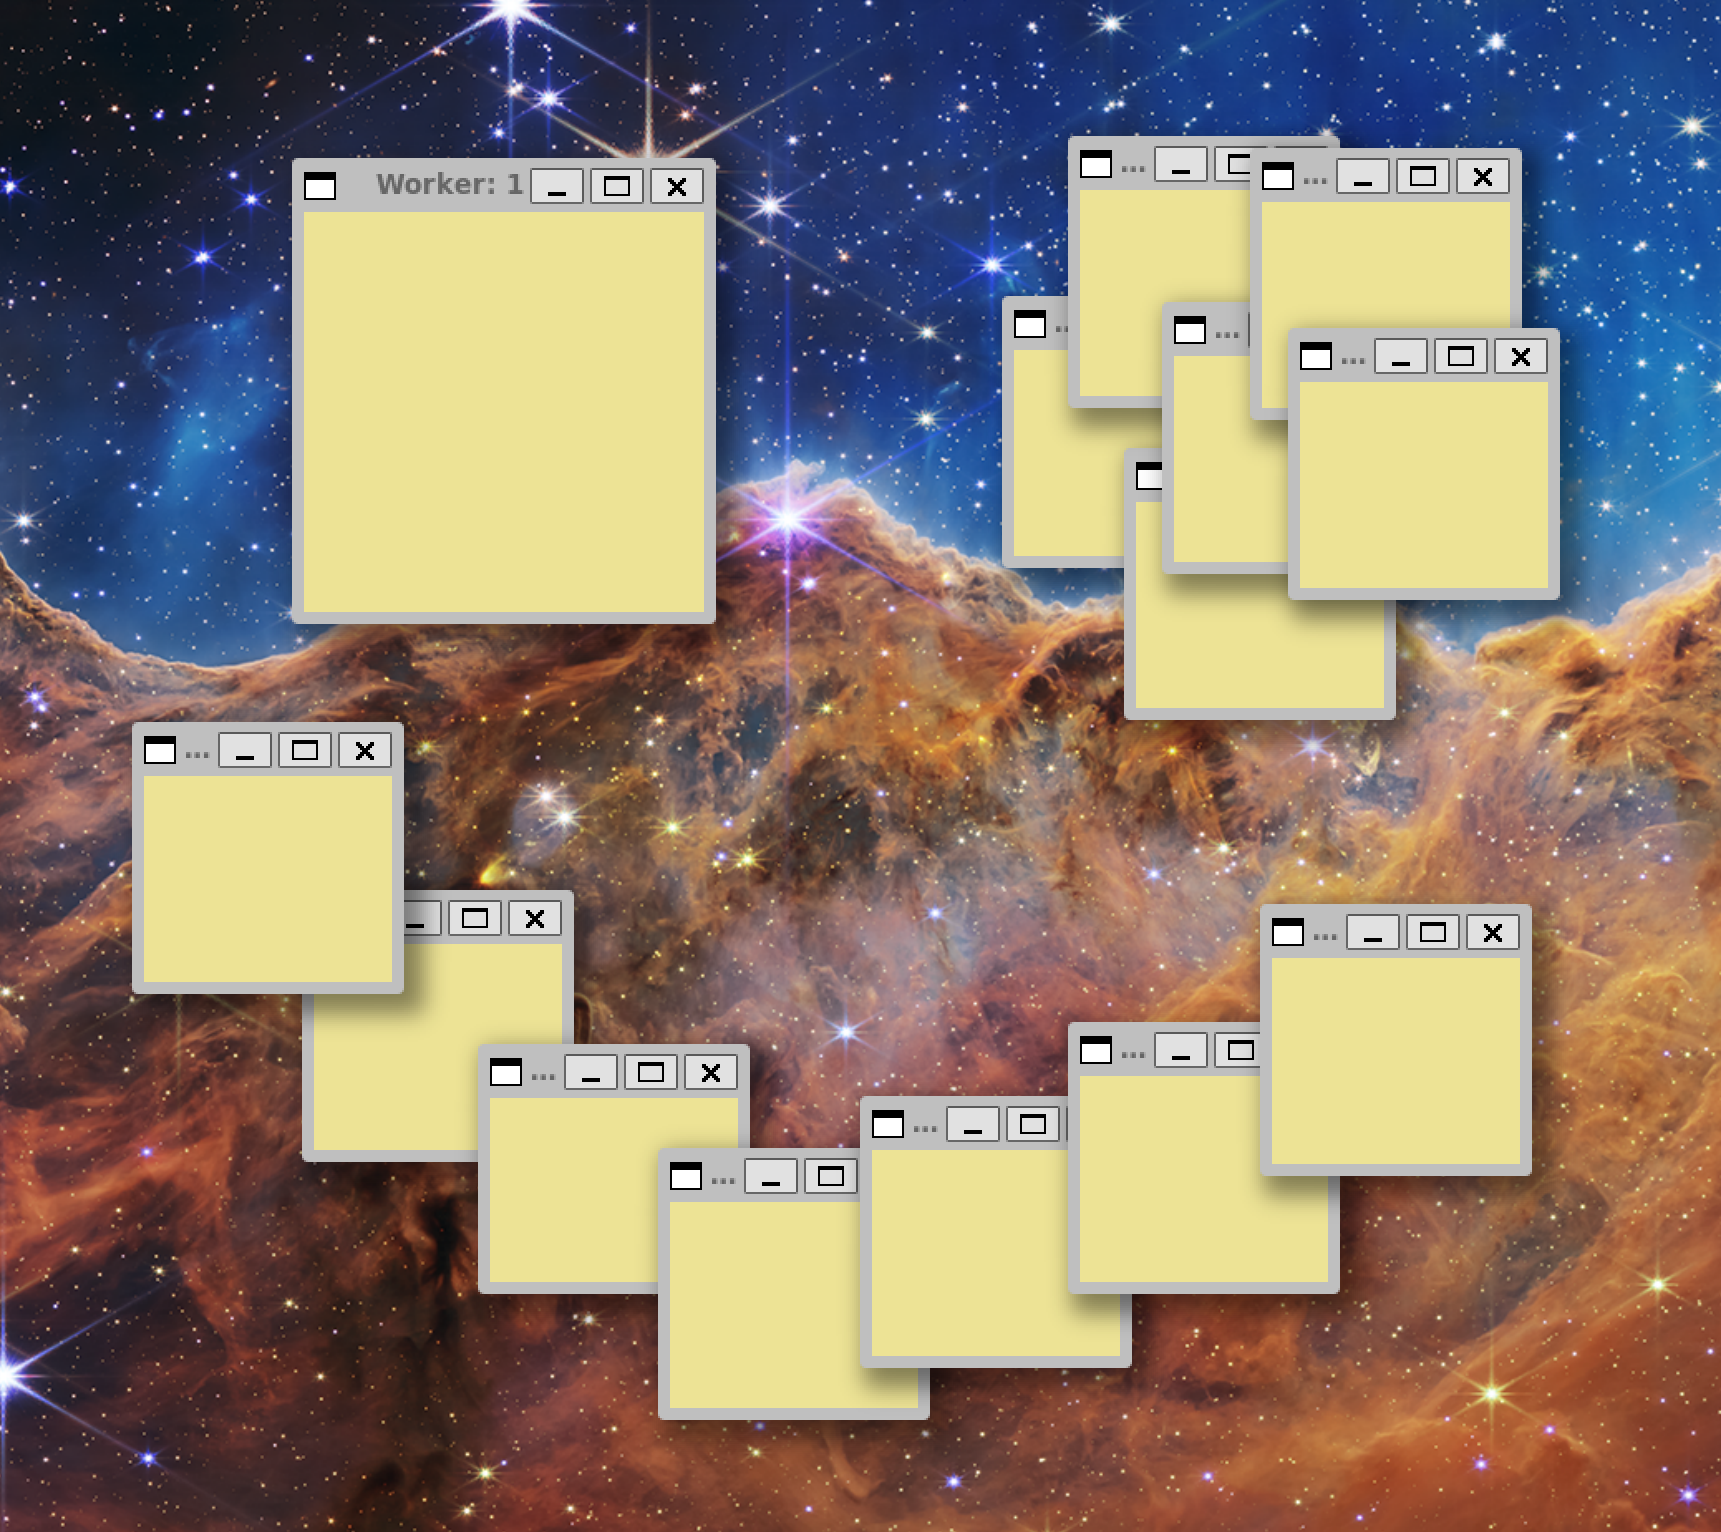
\includegraphics[width=0.7\textwidth]{imgs/processes_having_fun.png}
  \caption{Processes having fun: synchronized group membership in action.}
  \label{fig:processes_having_fun}
\end{figure}

\end{document}